\level{2}{Processo di documentazione}
	\level{3}{Attività}
	L'attività di documentazione è un'attività di supporto allo sviluppo fondamentale ai fini del progetto.
	L'assegnazione delle stesure dei diversi documenti viene fatta dal \insrole{Responsabile di Progetto} ai diversi membri del gruppo in considerazione dei diversi ruoli che essi ricoprono.
	La stesura dei documenti deve essere fatta nel modo più accurato e completo possibile, in modo da ridurre i tempi nella fase di verifica.
	\level{3}{Norme}
		\level{4}{Struttura dei documenti}
			Tutti i documenti ufficiali, ad eccezione dei \hyperref[sec:verbali]{verbali}, dovranno possedere la seguente struttura:
			\begin{enumerate}
				\item frontespizio;
				\item informazioni sul documento;
				\item diario delle modifiche;
				\item indice delle sezioni;
				\item indice delle tabelle;
				\item indice delle figure;
				\item introduzione;
				\item contenuto.
			\end{enumerate}
			L’ordine in cui le sezioni devono comparire all’interno di ciascun documento è fissato. La numerazione delle prime pagine dovrà essere rappresentata tramite cifre romane, mentre dall'introduzione in seguito dovranno essere utilizzate le cifre arabe. \\
			Di seguito viene descritto il contenuto di sezione.
			\level{5}{Frontespizio}
				La prima pagina di ogni documento contiene:
				\begin{enumerate}
					\item informazioni sul gruppo:
					\begin{enumerate}
						\item nome;
						\item logo;
						\item mail;
						\item sito web;
					\end{enumerate}
					\item informazioni sul progetto:
					\begin{enumerate}
						\item nome;
						\item azienda proponente;
					\end{enumerate}
					\item informazioni sul documento:
					\begin{enumerate}
						\item nome;
						\item versione.
					\end{enumerate}
				\end{enumerate}
			\level{5}{Informazioni sul documento}
				Questa sezione contiene le principali informazioni sul documento. In particolare, sono indicati:
				\begin{enumerate}
					\item versione;
					\item data di redazione;
					\item cognome e nome di coloro che hanno redatto il documento (in ordine alfabetico);
					\item cognome e nome di coloro che hanno verificato il documento (in ordine alfabetico);
					\item cognome e nome di colui che ha approvato il documento (Responsabile di Progetto);
					\item uso (interno o esterno);
					\item cognome e nome di coloro ai quali verrà distribuito il documento (in ordine alfabetico).
				\end{enumerate}
			\level{5}{Diario delle modifiche}
				Questa sezione descrive tramite una tabella le modifiche che sono state apportate al documento. Ogni riga del diario contiene:
				\begin{enumerate}
					\item versione del documento;
					\item data della modifica;
					\item cognome e nome degli autori della modifica (in ordine alfabetico);
					\item ruoli degli autori della modifica;
					\item sommario delle modifiche apportate.
				\end{enumerate}
				La tabella è ordinata in modo tale che le ultime modifiche appaiano nelle prime righe del diario delle modifiche.
			\level{5}{Indice}
				In tale sezione è presente l’indice. In esso sono contenuti:
				\begin{enumerate}
					\item elenco degli argomenti trattati all’interno del documento;
					\item pagine alle quali tali argomenti possono essere trovati.
				\end{enumerate}
			\level{5}{Indice delle tabelle}
				In tale sezione è presente l’indice delle tabelle. In esso sono contenuti:
				\begin{enumerate}
					\item elenco dei titoli delle tabelle presenti all’interno del documento;
					\item pagine alle quali le tabelle possono essere trovate.
				\end{enumerate}
				Nel caso in cui non siano presenti tabelle questa sezione può essere omessa.
			\level{5}{Indice delle figure}
				In tale sezione è presente l’indice delle figure. In esso sono contenuti:
				\begin{enumerate}
					\item elenco dei titoli delle figure presenti all’interno del documento;
					\item pagine alle quali le figure possono essere trovate.
				\end{enumerate}
				Nel caso in cui non siano presenti figure questa sezione può essere omessa.
			\level{5}{Introduzione}
				Tale sezione contiene quanto segue:
				\begin{enumerate}
					\item scopo del documento;
					\item glossario;
					\item riferimenti utili:
					\begin{enumerate}
						\item riferimenti normativi;
						\item riferimenti informativi.
					\end{enumerate}
				\end{enumerate}
			\level{5}{Contenuto}
				Va infine incluso il contenuto del documento. Questo deve essere propriamente suddiviso in sezioni e sottosezioni, secondo la gerarchia presente all’interno dell’indice analitico.
		\level{4}{Norme tipografiche}
			\level{5}{Formattazione generale}
				\level{6}{Testatine}
					Ogni pagina (eccetto il frontespizio) di ogni documento deve prevedere una testatina. In essa saranno sempre presenti i seguenti elementi:
					\begin{itemize}
						\item logo del team, posizionato a sinistra;
						\item nome del documento, posizionato a destra.
					\end{itemize}
				\level{6}{Piè di pagina}
					Ogni pagina (eccetto il frontespizio) di ogni documento deve prevedere un piè di pagina. In esso saranno sempre presenti i seguenti elementi:
					\begin{itemize}
						\item numero di pagina, posizionato al centro.
					\end{itemize}
				\level{6}{Orfani e vedove}
					E’ considerato sgradevole che una pagina finisca con la prima riga di un paragrafo (vedova) o che inizi con l’ultima riga di un paragrafo (orfano). Tali righe preferibilmente non dovranno essere presenti in alcun documento.
			\level{5}{Caratteri}
				\level{6}{Virgolette}
					L’uso delle virgolette inglesi (aperte: “; chiuse: ”) è previsto nei seguenti casi:
					\begin{itemize}
						\item riferimento al nome di un file;
						\item riferimento nome di un comando;
						\item riferimento a una parola in quanto tale.
					\end{itemize}
					In letteratura esse sono usate anche per parole utilizzate al di fuori del significato letterale e per espressioni gergali. Non sono previsti questi casi all’interno dei documenti, essendo l’uso di questo tipo di parole vietato (esse possono essere soggette a interpretazione personale).\\
					L’uso delle virgolette italiane (aperte «; chiuse: ») è previsto nei casi in cui si deve:
					\begin{itemize}
						\item citare una frase;
						\item citare un discorso diretto.
					\end{itemize}
					L’uso delle virgolette inglesi semplici (aperte: ‘; chiuse: ’) è previsto nei seguenti casi:
					\begin{itemize}
						\item riferimento a un singolo carattere;
					\end{itemize}
				\level{6}{Parentesi}
					L’uso delle parentesi tonde è previsto nei seguenti casi:
					\begin{itemize}
						\item puntualizzazioni;
						\item esempi.
					\end{itemize}
					L’uso delle parentesi quadre è previsto nei seguenti casi:
					\begin{itemize}
						\item riferimento a uno standard ISO.
					\end{itemize}
				\level{6}{Segni d'interpunzione}
					Ogni documento dovrà essere conforme alle seguenti norme:
					\begin{itemize}
						\item tutti i segni di interpunzione necessitano di uno spazio dopo, mai prima;
						\item non si usa mai il punto alla fine di un titolo;
						\item i puntini di sospensione non vengono utilizzati né all’inizio né alla fine delle citazioni, le quali sono per loro natura incomplete;
						\item quando si usano le parentesi, i segni di punteggiatura vanno dopo la loro chiusura (fatta eccezione per punti esclamativi, punti interrogativi e punti di sospensione legati logicamente al testo contenuto nelle parentesi);
						\item le parentesi non sono mai precedute da segni di interpunzione;
						\item se una parola abbreviata si trova alla fine della frase non va ripetuto il punto.
					\end{itemize}
				\level{6}{Numeri}
					I numeri andranno formattati secondo lo standard [SI/ISO 31-0]. Esso prevede che essi debbano essere formattati secondo le seguenti regole:
					\begin{itemize}
						\item per separare la parte intera dalla parte frazionaria si usa la virgola.
						\item se la parte intera di un numero possiede più di tre cifre, esse vanno separate in gruppi di tre partendo dal separatore decimale e andando verso sinistra. Per separare tali gruppi di cifre va utilizzato lo spazio unificatore e non lo spazio normale: esso è ottenuto tramite la combinazione di tasti alt+0160.
					\end{itemize}
			\level{5}{Stile del testo}
				\level{6}{Grassetto}
					Tale stile va applicato ai seguenti elementi:
					\begin{itemize}
						\item titoli (qualunque sia il livello di annidamento);
						\item nomi delle revisioni;
						\item nomi delle fasi di progetto;
						\item parola chiave di un elenco puntato o numerato.
					\end{itemize}
				\level{6}{Corsivo}
					Tale stile va applicato ai seguenti elementi:
					\begin{itemize}
						\item nomi di documenti;
						\item nomi di ruoli;
						\item parole da mettere in rilievo.
					\end{itemize}
				\level{6}{Sottolineato}
					Tale stile va applicato ai seguenti elementi:
					\begin{itemize}
						\item parole che sono punto focale dell’argomento.
					\end{itemize}
				\level{6}{Glossario}
					Tale stile va applicato ai seguenti elementi:
					\begin{itemize}
						\item parole presenti all’interno del glossario.
					\end{itemize}
				\level{6}{Monospace}
					Tale stile va applicato ai seguenti elementi:
					\begin{itemize}
						\item parti di codice;
						\item comandi;
						\item indirizzi web;
						\item nomi di file;
						\item percorsi (path).
					\end{itemize}
			\level{5}{Composizione del testo}
				\level{6}{Elenchi}
					L’elenco numerato va utilizzato quando conta l’ordine in cui gli elementi sono mostrati. Nell’utilizzarlo si seguono le seguenti norme:
					\begin{enumerate}
						\item al primo livello si utilizzano i numeri interi a partire da 1;
						\item al secondo livello si utilizzano le lettere dell’alfabeto a partire da ‘a’.
					\end{enumerate}
					L’elenco puntato va utilizzato quando non conta l’ordine in cui gli elementi sono mostrati. Nell’utilizzarlo si seguono le seguenti norme:
					\begin{enumerate}
						\item al primo livello si utilizzano i cerchi pieni (neri);
						\item al secondo livello si utilizzano i trattini.
					\end{enumerate}
					Inoltre, qualsiasi tipo di elenco deve rispettare le seguenti norme:
					\begin{itemize}
						\item se è presente almeno un elemento al cui interno è possibile trovare un ‘.’ allora si pone ‘.’ alla fine di tutti gli elementi. In alternativa si usa il ‘;’ per tutti gli elementi (tranne l’ultimo). Se è presente un elenco annidato c’è la possibilità di utilizzare ‘:’ alla fine dell’elemento.
						\item l’ultimo elemento di un elenco termina sempre con il ‘.’.
						\item la prima lettera degli elementi dell’elenco è sempre maiuscola, tranne nel caso in cui l’elenco è preceduto da ‘:’.
					\end{itemize}
				\level{6}{Descrizioni}
					Se si vuole strutturare una descrizione sotto forma di elenco, si deve utilizzare il costrutto \LaTeX{} \textbackslash begin\{description\} \textbackslash item [etichetta] \textbackslash end\{description\}.
				\level{6}{Note a piè di pagina}
					Rispettare le seguenti norme nella stesura e utilizzo delle note a piè di pagina:
					\begin{itemize}
						\item ogni nota dovrà iniziare con una lettera maiuscola;
						\item ogni nota dovrà terminare con il simbolo ‘.’;
						\item se una stessa nota viene utilizzata più volte all’interno di uno stesso documento, essa dovrà essere scritta solo una volta.
					\end{itemize}
			\level{5}{Formati ricorrenti} \label{sec:formatiricorrenti}
				\level{6}{Date}
					Le date devono essere espresse seguendo il formalismo indicato dallo standard [ISO~8601]: AAAA-MM-GG. Tale formalismo va interpretato nel seguente modo:
					\begin{enumerate}
						\item AAAA rappresenta l’anno;
						\item MM rappresenta il mese;
						\item GG rappresenta il giorno.
					\end{enumerate}
					Affinché tale formalismo venga seguito correttamente, per fare riferimento a una data si deve utilizzare il comando \LaTeX{} \textbackslash insdate\{giorno\}\{mese\}\{anno\}. Esso garantisce la corretta scrittura delle date.
				\level{6}{Orari}
					Gli orari devono essere espressi seguendo il formalismo indicato dallo standard [ISO 8601]: HH-MM. Tale formalismo va interpretato nel seguente modo:
					\begin{enumerate}
						\item HH rappresenta le ore (formato 24 ore);
						\item MM rappresenta i minuti.
					\end{enumerate}
					Affinché tale formalismo venga seguito correttamente, per fare riferimento a un orario si deve utilizzare il comando \LaTeX{} \textbackslash instime\{ore\}\{minuti\}. Esso garantisce la corretta scrittura degli orari.
				\level{6}{URI}
					Per fare riferimento a un URI è necessario utilizzare il comando \LaTeX{} apposito: \textbackslash insuri\{nome\_uri\}. Esso garantisce la corretta scrittura dell'URI secondo le norme seguenti:
					\begin{itemize}
						\item si adotta lo stile monospace;
						\item il testo è formattato tramite il colore blu.
					\end{itemize}
				\level{6}{Path}
					Per fare riferimento a un path è necessario utilizzare il comando \LaTeX{} apposito: \textbackslash inspath\{percorso\}. Esso garantisce la corretta scrittura del path secondo le norme seguenti:
					\begin{itemize}
						\item si adotta lo stile monospace.
					\end{itemize}
				\level{6}{Ruoli di progetto}
					Per fare riferimento a un ruolo di progetto è necessario utilizzare il comando \LaTeX{} apposito: \textbackslash insrole\{nome\_ruolo\}. Esso garantisce la corretta scrittura del ruolo secondo le norme seguenti:
					\begin{itemize}
						\item la prima lettera di ogni parola è maiuscola, eccetto le preposizioni;
						\item si adotta lo stile corsivo.
					\end{itemize}
				\level{6}{Nomi dei documenti}
					Per fare riferimento a un documento è necessario utilizzare il comando \LaTeX{} apposito: \textbackslash insdoc\{nome\_documento\}. Esso garantisce la corretta scrittura del documento secondo le norme seguenti:
					\begin{itemize}
						\item la prima lettera di ogni parola è maiuscola, eccetto le preposizioni;
						\item si adotta lo stile corsivo;
						\item il nome del documento va racchiuso tra virgolette inglesi (aperte: “; chiuse:”).
					\end{itemize}
					Se si vuole includere il numero nella forma X.Y che indica l’ultima versione del documento che si sta scrivendo, si deve utilizzare il comando \LaTeX{} \textbackslash lastversion\{\}.
				\level{6}{Nomi dei file}
					Per fare riferimento a un file è necessario utilizzare il comando \LaTeX{} apposito: \textbackslash insfile\{nome\_file\}. Esso garantisce la corretta scrittura del file secondo le norme seguenti:
					\begin{itemize}
						\item si adotta lo stile monospace;
						\item il nome del file va racchiuso tra virgolette inglesi (aperte: “; chiuse:”).
					\end{itemize}
				\level{6}{Revisioni}
					Per fare riferimento a una revisione è necessario utilizzare il comando \LaTeX{} apposito: \textbackslash insrev\{nome\_revisione\}. Esso garantisce la corretta scrittura della revisione secondo le norme seguenti:
					\begin{itemize}
						\item la prima lettera di ogni parola è maiuscola, eccetto le preposizioni;
						\item si adotta lo stile grassetto.
					\end{itemize}
				\level{6}{Fasi del progetto}
					Per fare riferimento a una fase di progetto è necessario utilizzare il comando \LaTeX{} apposito: \textbackslash insphase\{nome\_fase\}. Esso garantisce la corretta scrittura della fase di progetto secondo le norme seguenti:
					\begin{itemize}
						\item la prima lettera di ogni parola è maiuscola, eccetto le preposizioni;
						\item si adotta lo stile grassetto.
					\end{itemize}
				\level{6}{Nome del gruppo}
					Quando si fa riferimento al nome del gruppo è necessario utilizzare il comando \LaTeX{} apposito: \textbackslash groupname\{\}. Esso garantisce la corretta scrittura del nome del gruppo.
				\level{6}{Nome del progetto}
					Quando si fa riferimento al nome del progetto è necessario utilizzare il comando \LaTeX{} apposito: \textbackslash projectname\{\}. Esso garantisce la corretta scrittura del nome del gruppo.
				\level{6}{Nome del proponente}
					Quando si fa riferimento al proponente è necessario utilizzare il comando \LaTeX{} apposito: \textbackslash proponente\{\}. Esso garantisce la corretta scrittura del suo nome.
				\level{6}{Nome del committente}
					Quando si fa riferimento al committente è necessario utilizzare il comando \LaTeX{} apposito: \textbackslash committente\{\}. Esso garantisce la corretta scrittura del suo nome.
				\level{6}{Nomi propri}
					Ogniqualvolta si intende utilizzare un nome proprio si deve scrivere prima il cognome e successivamente il nome.\\
					Quando si parla di disporre i nomi in ordine alfabetico si da sempre per scontato che la prima lettera rispetto alla quale si ordina è la prima lettera del cognome.
				\level{6}{Sigle}\label{sec:sigle}
					Esistono delle sigle che servono per riferirsi velocemente a nomi di documenti, ruoli e a revisioni programmate. Esse sono le seguenti:
					\begin{itemize}
						\item ADR (Analisi Dei Requisiti);
						\item GL (Glossario);
						\item LDP (Lettera di presentazione);
						\item NDP (Norme Di Progetto);
						\item PDP (Piano Di Progetto);
						\item PDQ (Piano Di Qualifica);
						\item SDF (Studio Di Fattibilità);
						\item ST (Specifica Tecnica);
						\item RA (Revisione Di Accettazione);
						\item RP (Revisione Di Progettazione);
						\item RQ (Revisione Di Qualifica);
						\item RR (Revisione Dei Requisiti);
						\item PM (Project Manager);
						\item Am (Amministratore);
						\item An (Analista);
						\item Pt (Progettista);
						\item Pm (Programmatore);
						\item Ve (Verificatore).
					\end{itemize}
					L’uso di tale sigle è permesso solo all’interno dei seguenti elementi:
					\begin{itemize}
						\item tabelle;
						\item diagrammi (immagini);
						\item didascalie di tabelle e immagini;
						\item note a piè di pagina.
					\end{itemize}
		\level{4}{Componenti grafiche}
			\level{5}{Immagini}
				L’inserimento di immagini all’interno di un qualsiasi documento è regolamentato dalle seguenti norme:
				\begin{itemize}
					\item gli unici formati ammessi sono il PDF e il PNG;
					\item tutte le immagini all’interno di un documento devono essere numerate in modo crescente;
					\item tutte le immagini all’interno di un documento devono essere accompagnate da una breve descrizione.
				\end{itemize}
				Per permettere un facile rintracciamento delle immagini presenti all’interno di un documento basta controllare l’indice delle immagini.
			\level{5}{Tabelle}
				L’inserimento di tabelle all’interno di un qualsiasi documento è regolamentato dalle seguenti norme:
				\begin{itemize}
					\item tutte le tabelle all’interno di un documento devono essere numerate in modo crescente;
					\item tutte le tabelle all’interno di un documento devono essere accompagnate da una breve descrizione.
				\end{itemize}
				Per permettere un facile rintracciamento delle tabelle presenti all’interno di un documento basta controllare l’indice delle tabelle.
		\level{4}{Tipologie dei documenti}
			\level{5}{Documenti informali}
				Un documento viene considerato informale dal momento stesso della sua creazione fino a quando non viene reso formale. Ciò accade dopo che il documento è stato approvato dal Responsabile Di Progetto. Notare che prima di essere approvato il documento deve essere sottoposto ad attività di verifica.\\
				Tutti i documenti informali sono da considerarsi ad esclusivo uso interno.
			\level{5}{Documenti formali}
				Un documento risulta formale quando viene approvato dal Responsabile Di Progetto. Solo i documenti formali possono essere forniti a soggetti esterni al team.\\
				Notare che eventuali modifiche a un documento formale rendono tale documento informale.
			\level{5}{Glossario}
				In tale documento saranno inserite le definizioni rigorose e concise di tutti quei termini che:
				\begin{itemize}
					\item sono delle sigle;
					\item riguardano argomenti tecnici;
					\item generano confusione o non sono ben conosciuti;
					\item possono essere soggetti a interpretazione personale.
				\end{itemize}
				Questo viene fatto affinché vi sia sempre un comune quadro di riferimento grazie al quale è possibile parlare senza fraintendimenti.\\
				Il Glossario cataloga i termini in ordine lessicografico e li raggruppa in base alla prima lettera. Questo per far si che essi siano facilmente reperibili.
			\level{5}{Verbali} \label{sec:verbali}
				Ogni incontro tra membri del team e/o soggetti esterni prevede che debba essere redatto un verbale. Il suo scopo è quello di trascrivere in modo sintetico ma fedele quanto avviene e quanto è detto durante le riunioni.\\
				I verbali non possono essere soggetti a modifiche.
				\level{6}{Riunione esterna}
					Per riunione esterna si intende un incontro programmato al quale partecipano i membri del team e delle persone esterne al team (che possono essere il committente o i proponenti). I verbali di queste riunioni sono documenti ufficiali, che possono avere un potenziale valore normativo o essere fonti di requisiti. In considerazione di ciò, si è ritenuto consono che la redazione di questi verbali avvenga seguendo regole precise.\\
					Esso è redatto da un incaricato che può variare di volta in volta, a seconda delle necessità e delle persone presenti all’incontro.\\
					I verbali esterni devono avere questa struttura:
					\begin{itemize}
						\item frontespizio;
						\item indice;
						\item una sezione intitolata “Estremi del verbale” dove sono riportati i seguenti dati:
						\begin{itemize}
							\item data;
							\item ora;
							\item durata;
							\item luogo (se non si tratta di incontro telematico);
							\item partecipanti (esterni e interni).
						\end{itemize}
						\item una sezione contenente le domande e le risposte fatte durante la riunione.
					\end{itemize}
				\level{6}{Riunione interna}
					Sebbene i verbali delle riunioni interne, sia ordinarie che straordinarie, siano ritenuti di carattere informale, anch'essi sono sottoposti ad alcune regole minime per quanto concerne il contenuto.  \\
					Questi documenti dovranno presentare la seguente struttura:
					\begin{itemize}
						\item frontespizio;
						\item introduzione;
						\item appello dei partecipanti;
						\item ordine del giorno;
						\item verbale della riunione;
						\item varie ed eventuali/aggiornamento.
					\end{itemize}
		\level{4}{Versionamento dei documenti} \label{sec:versioni}
			Ogni tipo di documento (tranne i verbali) è sottoposto a versionamento. La versione di un documento avanza ogniqualvolta viene fatta una modifica (ovvero quando viene aggiornata la tabella delle modifiche).\\
			La versione di un documento viene indicata con la seguente sintassi: vX.YY. Tali lettere vanno interpretate nel seguente modo:
			\begin{itemize}
				\item ‘v’ è un carattere che indica la parola “versione”, esso rimane inalterato;
				\item X è un numero che indica quante volte il documento in esame è stato formalizzato;
				\item YY è un numero di due cifre che indica quante modifiche sono avvenute a partire dall’ultima formalizzazione del documento.
			\end{itemize}
			L’avanzamento di versione avviene nel seguente modo:
			\begin{enumerate}
				\item X parte da 0 e non ha limiti superiori. Esso viene incrementato di 1 ogni volta che il \insrole{Responsabile di Progetto} formalizza il documento.
				\item YY parte da 00 e non ha limiti superiori. Esso viene incrementato di 1 ogni volta che viene apportata una modifica al documento e viene riportato a 00 ogni volta che il documento è stato formalizzato.
			\end{enumerate}
			La prima versione di ogni documento è la v0.01.
	\level{3}{Procedure}
		\level{4}{Procedura di formalizzazione dei documenti}
			Di seguito viene riportata la procedura alla quale deve essere sottoposto un documento prima di essere definitivamente formalizzato:
			\begin{enumerate}
				\item i Redattori si occupano della stesura del documento e della correzione di eventuali errori (documento in lavorazione);
				\item il \insrole{Responsabile di Progetto} assegna a uno o più Verificatori il compito di verificare che non vi siano errori nella versione consegnata dai redattori (documento in verifica);
				\item se i Verificatori trovano degli errori, si torna al primo punto; se invece non viene rilevata alcuna anomalia il documento viene consegnato al \insrole{Responsabile di Progetto};
				\item il \insrole{Responsabile di Progetto} può decidere di approvare il documento (e in questo caso la procedura di formalizzazione termina, documento approvato) oppure di respingerlo (in questo caso si torna al primo punto).
			\end{enumerate}
			La procedura è formalizzata nel seguente diagramma delle attività:
			\begin{figure}[H]
				\centering
				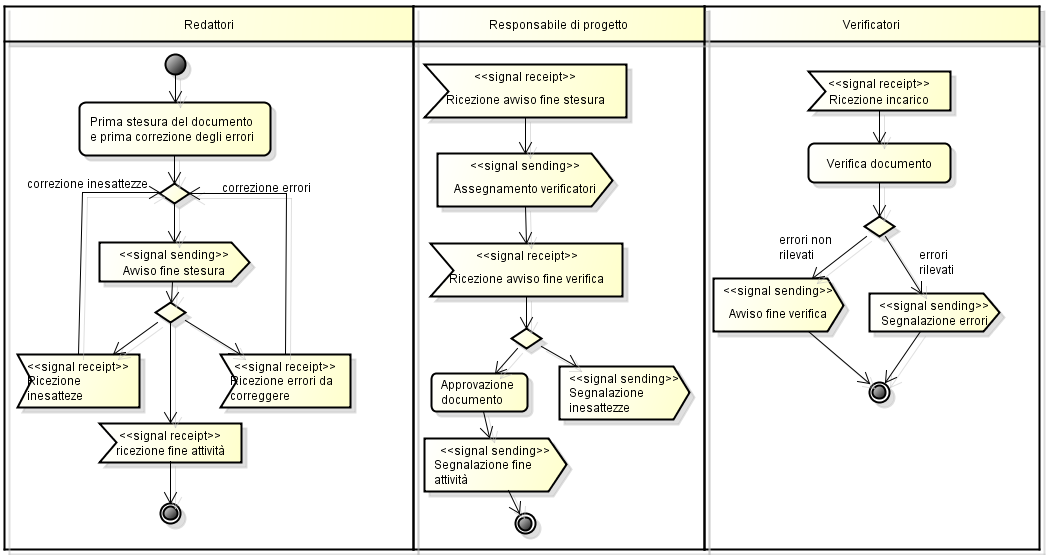
\includegraphics[width=0.6\textwidth]{NormeDiProgetto/Pics/FormalizzazioneDocumenti}
				\caption{Procedura di formalizzazione dei documenti}
			\end{figure}
	\level{3}{Strumenti}
		\level{4}{\LaTeX{}}
			Per la stesura dei documenti si è scelto di utilizzare il linguaggio di markup \LaTeX{}.  Il motivo principale che ha portato a questa scelta è la facilità di separazione tra contenuto e formattazione. Con \LaTeX{} è possibile scrivere testo senza doversi preoccupare di dare a esso una formattazione coerente con le norme: è infatti possibile definire un unico template, valido per qualsiasi documento, che applica le regole tipografiche in automatico.
			\level{5}{Template}
				Ogni documento dovrà essere realizzato a partire da un template \LaTeX{} appropriato reperibile al percorso Commons/Template.\\
				Grazie ai template di \LaTeX{}, non ci si deve preoccupare della formattazione del testo durante la sua stesura: infatti, basta impostare le regole all’interno di un unico file e queste verranno adottate in automatico all’interno di tutti i documenti che fanno uso del template. Inoltre, se le regole dovessero cambiare in corso d’opera (cambiamenti alle \insdoc{Norme di Progetto}), basta modificare il singolo file contenente le regole invece che tutti i documenti scritti fino a quel determinato momento.
			\level{5}{Comandi personalizzati}
				Per permettere un’adeguazione automatica alle regole imposte all’interno delle norme tipografiche si è deciso di creare dei comandi personalizzati utilizzabili in \LaTeX{}. Ogni membro del gruppo dovrà saperli usare in modo appropriato ogniqualvolta ve ne sia il bisogno.\\
				L’elenco completo di tutti i comandi lo si può trovare al punto \nameref{sec:formatiricorrenti};
		\level{4}{Strumenti per la rilevazione di errori ortografici}
			Per la rilevazione e la correzione di errori ortografici viene usato uno script creato dal gruppo \groupname{} che si appoggia al software Aspell, opportunamente configurato col dizionario di lingua italiana.
